\documentclass{beamer}

\usepackage{amsmath}
\usepackage{amsfonts}
\usepackage{amssymb}
\usepackage{graphicx}
\usepackage{listings}
\usepackage{color}

\hypersetup{
  colorlinks = true,
  linkcolor = blue,
  urlcolor = blue,
  citecolor = blue,
  anchorcolor = blue
}

\definecolor{lightgray}{rgb}{.9,.9,.9}
\definecolor{darkgray}{rgb}{.4,.4,.4}
\definecolor{darkgreen}{rgb}{0,0.4,0}

\lstdefinelanguage{JavaScript}{
    keywords={typeof, new, true, false, catch, function, return, null, catch, switch, var, if, in, while, do, else, case, break},
    keywordstyle=\color{blue}\bfseries,
    ndkeywords={class, export, boolean, throw, implements, import, this},
    ndkeywordstyle=\color{darkgray}\bfseries,
    identifierstyle=\color{black},
    sensitive=false,
    comment=[l]{//},
    morecomment=[s]{/*}{*/},
    commentstyle=\color{darkgreen}\ttfamily,
    stringstyle=\color{red}\ttfamily,
    morestring=[b]',
    morestring=[b]"
}

\lstset{
    language=JavaScript,
    backgroundcolor=\color{lightgray},
    extendedchars=true,
    basicstyle=\tiny\ttfamily,
    showstringspaces=false,
    showspaces=false,
    tabsize=2,
    breaklines=true,
    showtabs=false,
    captionpos=b
}

\usepackage{polski}
\usepackage[polish]{babel}
\usepackage[utf8]{inputenc}

\begin{document}

  \begin{frame}
    \begin{center}
      
\includegraphics[width=\textwidth,keepaspectratio]{img/logo.png}

      Dawid Czech, Marcin Radomski
    \end{center}
  \end{frame}

  \begin{frame}
    \frametitle{Model danych}
    \begin{columns}
      \column{.6\textwidth}
      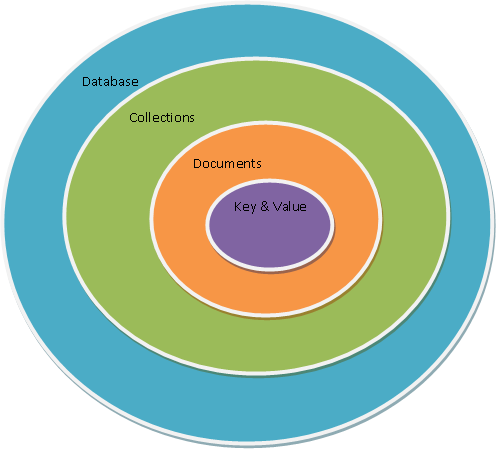
\includegraphics[scale=0.5]{img/db-structure.png}

      \column{.4\textwidth}
      Dane w MongoDB są przechowywane jako zbiór \emph{par klucz-wartość}, pogrupowanych w \emph{dokumenty}. Wiele dokumentów tworzy \emph{kolekcję}, a zbiór kolekcji to właściwa \emph{baza}.
    \end{columns}
  \end{frame}

  \begin{frame}
    \frametitle{Dokument}
    Dane znajdujące się w dokumencie są zapisywane jako obiekty w formacie BSON (Binary JSON), który definiuje nie tylko typy prymitywne jak liczba czy tekst, ale również tablice czy podobiekty:
    \lstinputlisting{listings/document.js}

    Więcej o formacie BSON: \url{http://bsonspec.org/}
  \end{frame}

  \begin{frame}
    \frametitle{Zalety}
    \begin{itemize}
      \item Łatwość tworzenia bazy
      \begin{itemize}
        \item Odwołanie do nieistniejącej kolekcji tworzy ją automatycznie
      \end{itemize}
      \item Brak określonej struktury danych w dokumencie
      \item Intuicyjna struktura danych w bazie
      \begin{itemize}
        \item Tablice, słowniki, nawet wyrażenia regularne
      \end{itemize}
      \item Konsola z interpreterem JavaScriptu
    \end{itemize}
  \end{frame}

  \begin{frame}
    \frametitle{Wady}
    \begin{itemize}
      \item Nie nadaje się do każdego rodzaju danych
      \item Brak określonej struktury danych w dokumencie...
      \begin{itemize}
        \item Konieczność używania indeksów
      \end{itemize}
      \item Konieczność przechowywania nazw pól w każdym dokumencie
      \begin{itemize}
        \item Ogromne marnotrawstwo pamięci w przypadku dużych baz
      \end{itemize}
      \item Duplikacja danych
      \item Niecodzienna składnia porównań w zapytaniach
    \end{itemize}
  \end{frame}

  \begin{frame}
    \frametitle{Dobry przykład}
  \end{frame}

  \begin{frame}
    \frametitle{Zły przykład}
  \end{frame}

  \begin{frame}
    \frametitle{CRUD}
    \begin{itemize}
      \item Select
      \lstinputlisting{listings/crud-select.js}
      \item Insert
      \lstinputlisting{listings/crud-insert.js}
      \item Update
      \lstinputlisting{listings/crud-update.js}
      \item Remove
      \lstinputlisting{listings/crud-remove.js}
    \end{itemize}
  \end{frame}

  \begin{frame}
    \frametitle{Filtrowanie dokumentów}
    \begin{itemize}
      \item \texttt{\{ klucz: 'wartość' \}} - 'jest równe'
      \item \texttt{\{ \$operator: argument(y) \}}
      \begin{itemize}
        \item \texttt{\{ \$lt: 20 \}} - 'mniejsze od'
        \item \texttt{\$gt, \$lte, \$gte, \$ne} - inne porównania
        \item \texttt{\{ \$in: [ 'A', 'B' ] \}} - 'należy do zbioru'
        \item \texttt{\$nin} - 'nie należy do zbioru'
      \end{itemize}
      \item Operatory logiczne:
      \begin{itemize}
        \item \texttt{\$and, \$or, \$nor, \$not}
        \item W przypadku podania kilku warunków wszystkie muszą być spełnione
      \end{itemize}
      \item Do stringów - wyrażenia regularne: \texttt{\{ name: /.*a.*/ \}}
    \end{itemize}
    \lstinputlisting{listings/find-basic.js}
  \end{frame}

  \begin{frame}
    \frametitle{Filtrowanie dokumentów - tablice i subdokumenty}
    \begin{itemize}
      \item Tablice
      \begin{itemize}
        \item \texttt{\{ tablica: [ 'A', 'B' ] \}} - dokładne dopasowanie
        \item \texttt{\{ tablica: 'A' \}} - czy tablica zawiera element 'A'?
        \item \texttt{\{ 'tablica.2': 'A' \}} - czy trzeci element tablicy to 'A'? (indeksowanie od 0)
        \item \texttt{\{ \$elemMatch: warunek \}} - wybieranie niektórych elementów tablicy
      \end{itemize}
      \item \texttt{\{ 'kot.kolor': 'czarny' \}} - sprawdzanie pola subdokumentu
      \lstinputlisting{listings/find-array-struct.js}
    \end{itemize}
  \end{frame}

  \begin{frame}
    \frametitle{Aggregation Framework}
    Aggregation Framework, będący częścią MongoDB pozwala na wykonywanie dowolnych operacji typu map-reduce.
  \end{frame}

  \begin{frame}
    \frametitle{SQL vs MongoDB}
    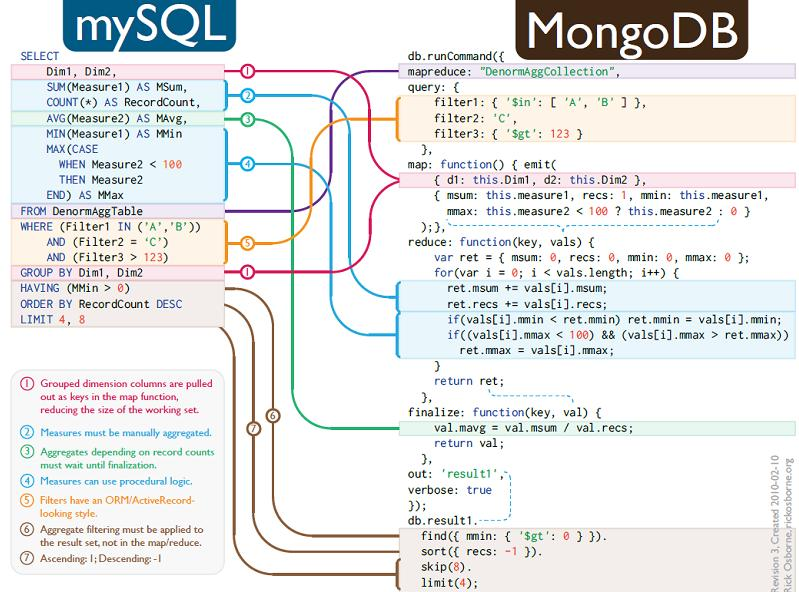
\includegraphics[width=\textwidth,keepaspectratio]{img/mysql_vs_mongodb.jpg}
  \end{frame}

  \begin{frame}
    \frametitle{MongoDB w NodeJS}
    \lstinputlisting{listings/node.js}
  \end{frame}

  \begin{frame}
    \frametitle{Instalacja: Linux}
    Wystarczy zainstalować odpowiednią paczkę z repozytorium. Dla Ubuntu sprowadza się to do wykonania:

    \lstinputlisting{listings/install-linux.sh}
  \end{frame}

  \begin{frame}
    \frametitle{Instalacja: Windows}
  \end{frame}

\end{document}
